\newpage
\textbf{\textcolor{MidnightBlue}{2.}}
Considera la ejecución de la figura 1. Haz lo siguiente:
\begin{enumerate}[a)]
%%%%%%%%%%%%%%%%%%%%%%%%%%%%        Inciso A        %%%%%%%%%%%%%%%%%%%%%%%%%%%%%%%%%%
\item Ejecuta el algoritmo de relojes lógicos y asigna el tiempo lógico a cada evento.
%%%%%%%%%%%%%%%%%%%%%%%%%%%%        Inciso B        %%%%%%%%%%%%%%%%%%%%%%%%%%%%%%%%%%
\item Ejecuta el algoritmo de relojes vectoriales y asigna el vector de tiempo
a cada evento.
%%%%%%%%%%%%%%%%%%%%%%%%%%%%        Inciso C        %%%%%%%%%%%%%%%%%%%%%%%%%%%%%%%%%%
\item Muestra dos cortes consistentes y dos inconsistentes.
\end{enumerate}
\begin{center}
    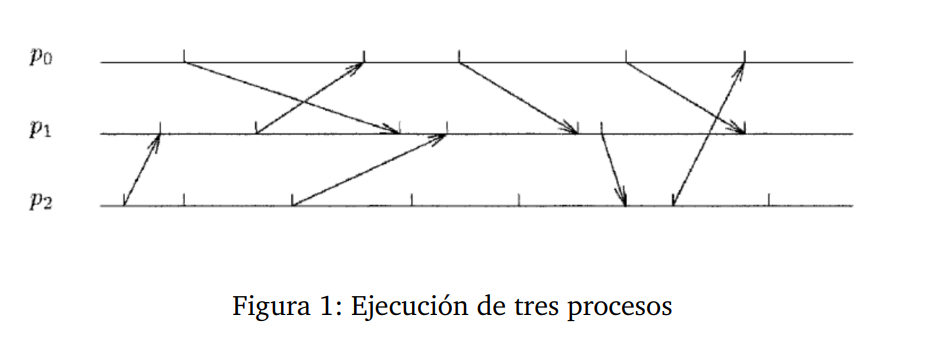
\includegraphics[scale=0.5]{Grapho.png}
\end{center}

$\rhd$ \textbf{Solución:} \newline
($a$) \textit{Relojes lógicos.} A continuación se muestra una ejecución del algoritmo con
      relojes lógicos:
      \begin{figure}[ht!]
        \begin{center}
                \begin{tikzpicture}
                        %% Conjunto de eventos P_0:
                        \node(P01)  [blueV, label=90:$1$]      at (2,0)  {};
                        \node(P02)  [blueV, label=90:$4$]      at (5,0)  {};
                        \node(P03)  [blueV, label=90:$5$]      at (7,0)  {};
                        \node(P04)  [blueV, label=90:$6$]      at (11,0) {};
                        \node(P05)  [blueV, label=90:$10$]     at (13.5,0) {};
                        %% Marca de tiempo de P_0:
                        \draw [edge]  (0,0) to (P01);
                        \draw [edge]  (P01) to (P02);
                        \draw [edge]  (P02) to (P03);
                        \draw [edge]  (P03) to (P04);
                        \draw [edge]  (P04) to (P05);
                        \draw [edge]  (P05)   to (14,0);
                        %% Conjunto de eventos P_1:
                        \node(P11)  [redV, label=90:$2$]      at (1,-1.5)    {};
                        \node(P12)  [redV, label=90:$3$]      at (3.5,-1.5)  {};
                        \node(P13)  [redV, label=90:$4$]      at (5.5,-1.5)  {};
                        \node(P14)  [redV, label=90:$5$]      at (6.5,-1.5)  {};
                        \node(P15)  [redV, label=90:$6$]      at (8.5,-1.5)  {};
                        \node(P16)  [redV, label=90:$7$]      at (9,-1.5)    {};
                        \node(P17)  [redV, label=90:$8$]      at (13.5,-1.5) {};
                        %% Marca de tiempo de P_1:
                        \draw [edge]  (0,-1.5) to (P11);
                        \draw [edge]  (P11)  to (P12);
                        \draw [edge]  (P12)  to (P13);
                        \draw [edge]  (P13)  to (P14);
                        \draw [edge]  (P14)  to (P15);
                        \draw [edge]  (P15)  to (P16);
                        \draw [edge]  (P16)  to (P17);
                        \draw [edge]  (P17)  to (14,-1.5);
                        %% Conjunto de eventos P_2:
                        \node(P21)  [yellowV, label=90:$1$]      at (0,-3)  {};
                        \node(P22)  [yellowV, label=90:$2$]      at (2,-3)  {};
                        \node(P23)  [yellowV, label=90:$3$]      at (4,-3)  {};
                        \node(P24)  [yellowV, label=90:$4$]      at (6,-3) {};
                        \node(P25)  [yellowV, label=90:$5$]      at (8,-3) {};
                        \node(P26)  [yellowV, label=90:$8$]      at (10,-3) {};
                        \node(P27)  [yellowV, label=90:$9$]      at (12,-3) {};
                        \node(P28)  [yellowV, label=90:$10$]     at (14,-3) {};
                        %% Marca de tiempo de P_2:
                        \draw [edge]  (P21) to (P22);
                        \draw [edge]  (P22) to (P23);
                        \draw [edge]  (P23) to (P24);
                        \draw [edge]  (P24) to (P25);
                        \draw [edge]  (P25) to (P26);
                        \draw [edge]  (P26) to (P27);
                        \draw [edge]  (P27) to (P28);
                        
                        %% Relacionando eventos locales de distintos procesos:
                        \draw [edge->]  (P01) to (P13);
                        \draw [edge->]  (P03) to (P15);
                        \draw [edge->]  (P04) to (P17);
                        \draw [edge->]  (P12) to (P02);
                        \draw [edge->]  (P16) to (P26);
                        \draw [edge->]  (P21) to (P11);
                        \draw [edge->]  (P23) to (P14);
                        \draw [edge->]  (P27) to (P05);
                        
                        %% Nombres de procesos:
                        \node(P0)  [label=90:$P_0$]      at (-1,-0.3)    {};
                        \node(P1)  [label=90:$P_2$]      at (-1,-1.8)    {};
                        \node(P2)  [label=90:$P_1$]      at (-1,-3.3)    {};
                \end{tikzpicture}
        \end{center}
      \end{figure}

($b$) \textit{Relojes Vectoriales.} A continuación se muestra una ejecución del algoritmo con relojes vectoriales:

      \begin{figure}[ht!]
        \begin{center}
                \begin{tikzpicture}
                        %% Conjunto de eventos P_0:
                        \node(P01)  [blueV, label=90:$(1\ 0\ 0)$]      at (2,0)  {};
                        \node(P02)  [blueV, label=90:$(2\ 2\ 1)$]      at (5,0)  {};
                        \node(P03)  [blueV, label=90:$(3\ 2\ 1)$]      at (7,0)  {};
                        \node(P04)  [blueV, label=90:$(4\ 2\ 1)$]      at (11,0) {};
                        \node(P05)  [blueV, label=90:$(5\ 6\ 7)$]     at (13.5,0) {};
                        %% Marca de tiempo de P_0:
                        \draw [edge]  (0,0) to (P01);
                        \draw [edge]  (P01) to (P02);
                        \draw [edge]  (P02) to (P03);
                        \draw [edge]  (P03) to (P04);
                        \draw [edge]  (P04) to (P05);
                        \draw [edge]  (P05)   to (14,0);
                        %% Conjunto de eventos P_1:
                        \node(P11)  [redV, label=90:$(0\ 1\ 1)$]      at (1,-1.5)    {};
                        \node(P12)  [redV, label=270:$(0\ 2\ 1)$]      at (3.5,-1.5)  {};
                        \node(P13)  [redV, label=90:$(1\ 3\ 1)$]      at (5.5,-1.5)  {};
                        \node(P14)  [redV, label=90:$(1\ 4\ 3)$]      at (6.5,-1.5)  {};
                        \node(P15)  [redV, label=270:$(3\ 5\ 3)$]      at (8.5,-1.5)  {};
                        \node(P16)  [redV, label=90:$(3\ 6\ 3)$]      at (9,-1.5)    {};
                        \node(P17)  [redV, label=270:$(4\ 7\ 3)$]      at (13.5,-1.5) {};
                        %% Marca de tiempo de P_1:
                        \draw [edge]  (0,-1.5) to (P11);
                        \draw [edge]  (P11)  to (P12);
                        \draw [edge]  (P12)  to (P13);
                        \draw [edge]  (P13)  to (P14);
                        \draw [edge]  (P14)  to (P15);
                        \draw [edge]  (P15)  to (P16);
                        \draw [edge]  (P16)  to (P17);
                        \draw [edge]  (P17)  to (14,-1.5);
                        %% Conjunto de eventos P_2:
                        \node(P21)  [yellowV, label=270:$(0\  0\ 1)$]    at (0,-3)  {};
                        \node(P22)  [yellowV, label=90:$(0\ 0\ 2)$]      at (2,-3)  {};
                        \node(P23)  [yellowV, label=270:$(0\ 0\ 3)$]     at (4,-3)  {};
                        \node(P24)  [yellowV, label=90:$(0\ 0\ 4)$]      at (6,-3) {};
                        \node(P25)  [yellowV, label=90:$(0\ 0\ 5)$]      at (8,-3) {};
                        \node(P26)  [yellowV, label=270:$(3\ 3\ 6)$]     at (10,-3) {};
                        \node(P27)  [yellowV, label=270:$(3\ 6\ 7)$]     at (12,-3) {};
                        \node(P28)  [yellowV, label=90:$(3\ 6\ 8)$]      at (14,-3) {};
                        %% Marca de tiempo de P_2:
                        \draw [edge]  (P21) to (P22);
                        \draw [edge]  (P22) to (P23);
                        \draw [edge]  (P23) to (P24);
                        \draw [edge]  (P24) to (P25);
                        \draw [edge]  (P25) to (P26);
                        \draw [edge]  (P26) to (P27);
                        \draw [edge]  (P27) to (P28);
                        
                        %% Relacionando eventos locales de distintos procesos:
                        \draw [edge->]  (P01) to (P13);
                        \draw [edge->]  (P03) to (P15);
                        \draw [edge->]  (P04) to (P17);
                        \draw [edge->]  (P12) to (P02);
                        \draw [edge->]  (P16) to (P26);
                        \draw [edge->]  (P21) to (P11);
                        \draw [edge->]  (P23) to (P14);
                        \draw [edge->]  (P27) to (P05);
                        
                        %% Nombres de procesos:
                        \node(P0)  [label=90:$P_0$]      at (-1,-0.3)    {};
                        \node(P1)  [label=90:$P_2$]      at (-1,-1.8)    {};
                        \node(P2)  [label=90:$P_1$]      at (-1,-3.3)    {};
                \end{tikzpicture}
        \end{center}
      \end{figure}

($c$) \textit{Corte consistente.}
\begin{figure}[h]
  \centering
  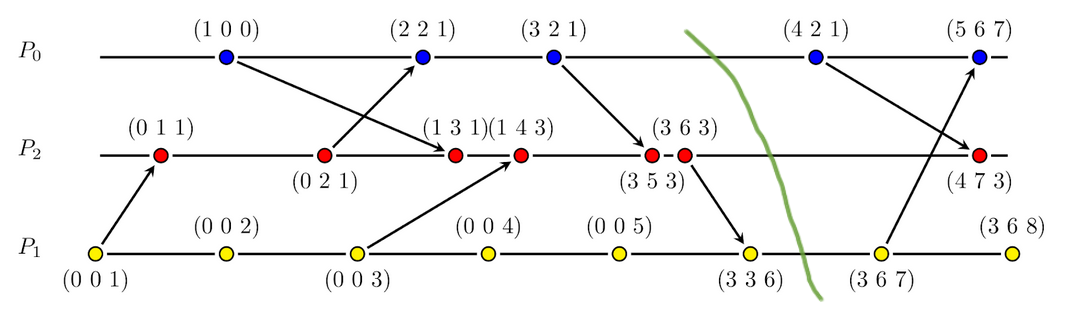
\includegraphics[scale=0.3]{./CorteConsistente.png}
  \caption{Corte Consistente.}
\end{figure}

($d$) \textit{Corte inconsistente.}
\begin{figure}[h]
  \centering
  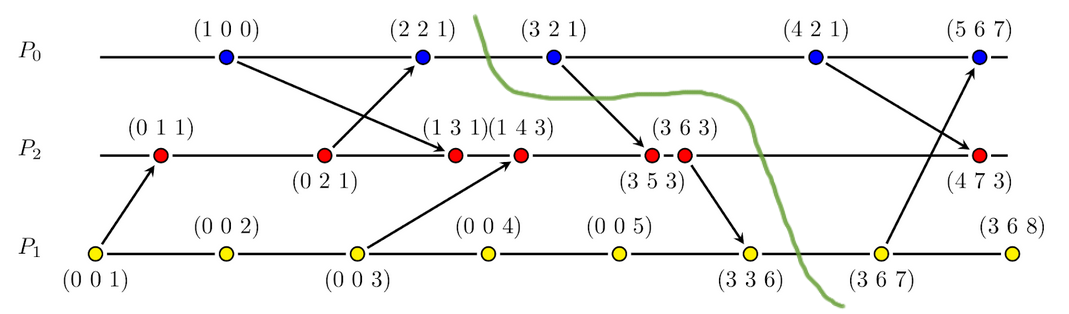
\includegraphics[scale=0.3]{./CorteInconsistente.png}
  \caption{Corte Consistente.}
\end{figure}
\newline

Como podemos notar, en ($d$) el corte inconsistente se da con base en el
tercer estado local de $P_0$.
\hfill $\lhd$
